\chapter{Replicação Ativa e Paxos}\label{cap1:replicacao_ativa_paxos}

Normalmente, uma aplicação distribuída é estruturada em termos de clientes e serviços.
Cada serviço suporta uma ou mais operações invocadas pelos clientes através de requisições
remotas. Embora o uso de um único servidor (computação centralizada) seja a maneira mais
simples para implementar um serviço, a confiabilidade desse serviço resultante está
diretamente ligada a tolerância a falhas do servidor. Se esse nível de tolerância é
inaceitável, então, a mesma versão desse serviço deve ser replicada em servidores
diferentes, visando mitigar os erros. O isolamento físico das unidades de processamento em
um sistema distribuído garante que as falhas serão independentes \cite{schneider90}.

Do ponto de vista de hardware, redundância é a técnica chave para tolerância a falhas e
alta disponibilidade. O princípio básico dessa técnica é que se um dos componentes
redundantes falha, os demais podem continuar o trabalho em seu lugar, gerando o mínimo de
interrupção do serviço. Criar um \emph{grupo de réplicas} para suportar a implementação de
um serviço minimiza a percepção de falhas do cliente. Entretanto, para que o grupo de
réplicas seja transparente ao cliente, é preciso adotar uma estratégia de replicação capaz
de coordenar as réplicas no momento que falham \cite{jalote94}.

A coordenação do hardware replicado é realizado por software, usando estratégias como
\emph{replicação ativa} capaz de tolerar falhas de maneira transparente visando o
progresso da aplicação. O princípio por trás da replicação ativa é a suposição de que cada
\emph{réplica} opera como uma máquina de estados determinista, de forma que elas
mantenham-se idênticas ao executarem as mesmas transições de estado, na mesma ordem
\cite{schneider90}. A consistência de atualização de dados é mantida por algum protocolo,
executado pelas réplicas, que permita difundir e ordenar totalmente essas transições.

Neste capítulo apresentamos os aspectos conceituais de aplicações que utilizam o modelo de
replicação ativa através do algoritmo Paxos, necessários para compreensão do restante do
trabalho. Na \autoref{sec:modelo-computacional}, começamos definindo conceitos
fundamentais sobre o modelo computacional adotado. A \autoref{sec:replicacao-ativa} examina
detalhadamente o modelo de replicação ativa e na \autoref{sec:paxos} descrevemos o
funcionamento do algoritmo Paxos e seus principais componentes. Em seguida, na
\autoref{sec:treplica} apresentamos a biblioteca Treplica que é uma implementação do
modelo de replicação ativa utilizando Paxos. Na \autoref{sec:reconfiguracao}, falamos dos
principais aspectos de reconfiguração em um sistema distribuído executando Paxos.
Finalmente, a \autoref{sec:trabalhos-relacionados} encerra o capítulo mostrando os
trabalhos relacionados a esta dissertação.


\section{Modelo Computacional}\label{sec:modelo-computacional}

Um sistema distribuído pode ser definido como um conjunto de réplicas autônomas,
interconectadas via rede, que se comunicam através de troca de mensagens. Para este
trabalho, adotamos o modelo modelo computacional \emph{falha-e-recuperação assíncrono}. As
premissas em relação às réplicas são: 1) réplicas passam por períodos de instabilidade e
falham, mas conseguem se recuperar, porém perdendo a sua memória volátil; 2) uma réplica é
considerada defeituosa se não consegue se recuperar mais ou se fica em um ciclo constante
de falha e recuperação \cite{cachin11}.

Essas réplicas trocam mensagens por um enlace de \emph{perda-justa}, que possui as
seguintes propriedades \cite{cachin11}:

\begin{itemize}
  \item Perda-justa: se um processo correto $p$ envia infinitas mensagens $m$ para um
    processo correto $q$, então $q$ entrega $m$ um número infinito de vezes;
  \item Duplicação finita: se um processo correto $p$ envia um número finito de vezes a
    mensagem $m$ para um processo correto $q$, então $m$ não pode ser entregue infinitas
    vezes por $q$; e
  \item Sem criação: se algum processo $q$ entrega a mensagem $m$ enviada pelo processo
    $p$, então $m$ foi anteriormente enviada de $p$ para $q$.
\end{itemize}

Enlaces de perda-justa podem ser implementados diretamente sobre uma rede de comunicação,
ou seja, a implementação da abstração não garante as propriedades, apenas percebe que elas
existem no substrato escolhido. O protocolo UDP é um exemplo de protocolo que implementa o
modelo perda-justa, na ausência de falhas graves. É importante ressaltar que a propriedade
que garante entrega de mensagens entre réplicas não é suportada pelo modelo de comunicação
perda-justa. Essa propriedade é inerente ao algoritmo Paxos.

Relacionado ao modelo computacional assíncrono, as seguintes premissas são relevantes: 1)
não existe limite a diferença de velocidade de processamento entre duas réplicas; 2) não
existe limite para a latência de transferência de uma mensagem. Então, podemos afirmar que
não existe nenhuma suposição de sincronia entre réplicas baseado nessas propriedades.

\subsection{Tolerância a Falhas}

Um componente é considerado defeituoso quando seu comportamento não está de acordo com sua
especificação \cite{schneider90}. Para tolerância a falhas, a perspectiva do usuário é a
mais importante. Por isso, gostaríamos que as aplicações distribuídas continuem
funcionando (progredindo) apesar das falhas \cite{jalote94}.

Os principais componentes de um sistema distribuído são: processadores, redes, relógios,
armazenamento não volátil e software. Normalmente esses componentes não são construídos
para suportar tolerância a falhas e são suas estruturas que utilizamos para apoiar os
mecanismos de tolerância a falhas. Exceto software, todos os outros componentes são
físicos e sua falha pode ter causas físicas subjacentes. Suportar por software falhas em
mecanismos físicos é o principal foco da maioria dos mecanismos de tolerância a falhas,
especialmente em servidores e redes de comunicação \cite{jalote94}.

Tais falhas podem ser classificadas de acordo com o comportamento defeituoso apresentado
no momento da falha \cite{jalote94}. Essa classificação pelo comportamento da falha
especifica quais pressupostos podem ser feitos sobre o comportamento do componente quando
ele falha. Uma dessas classificações é dada por \citeonline{cristian86}, onde cada falha
pertence a uma de quatro categorias: Acidente (\emph{Crash}), Omissão (\emph{Omission}),
Tempo (\emph{Timing}) ou Bizantina (\emph{Byzantine}).

\begin{itemize}
  \item Falha por Acidente: esta falha faz com que a réplica paralise o perca seu estado
    interno. Esse tipo de falha nunca leva o componente a sofrer uma transição de estado
    incorreta quando ele falha.
  \item Falha por Omissão: ocorre quando a réplica deixa de responder a algumas
    requisições enviadas a ela. Quando a réplica falha por omissão e deixa de responder
    indefinidamente, considera-se que a semântica da falha é silenciosa~\cite{cristian91}.
  \item Falha por Tempo: quando uma réplica responde uma requisição demasiadamente tarte é
    classificada como falha por tempo.
  \item Falha Bizantina: ocorre quando não é feita nenhuma restrição quanto ao
    comportamento falho da réplica. Nessa semântica, a réplica pode deixar de responder,
    atrasar envio de respostas, enviar respostas erradas, enviar respostas diferentes para
    diferentes destinos, recusar o recebimento de requisições ou ainda, maliciosamente,
    fazer se passar por outra réplica~\cite{jalote94}.
\end{itemize}

Esse grupo de falhas formam uma hierarquia, sendo a falha por acidente a mais simples e
restritiva (ou bem definida) e a falha Bizantina a menos restritiva \cite{jalote94}. A
relação de inclusão é ilustrada na \autoref{fig:fault-classification} \cite{cristian86}:

\begin{figure}[htbp]
  \centering
  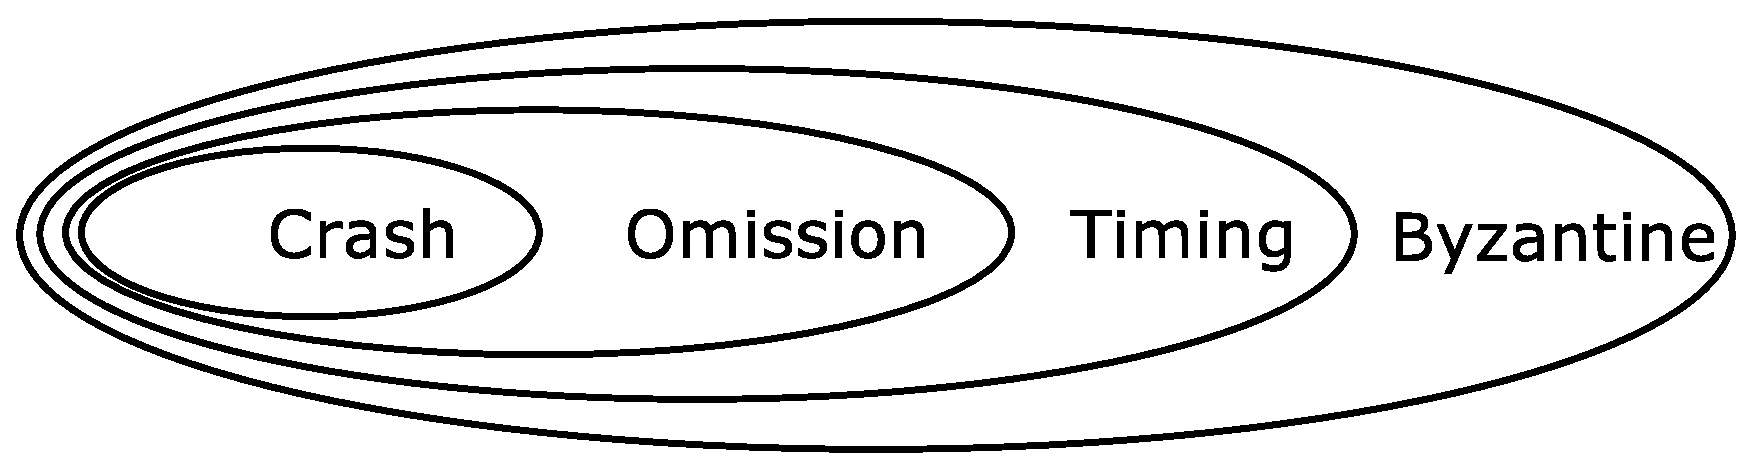
\includegraphics[width=13cm]{conteudo/capitulos/figuras/classificacao_falhas.eps}
  \caption{Classificação de falhas}
  \label{fig:fault-classification}
\end{figure}

Projetamos sistemas distribuídos tolerantes a falhas para fornecer um serviço confiável e
contínuo, apesar das falhas de alguns de seus componentes. Um mecanismo básico utilizado
na construção é o \emph{detector de falhas}, que a grosso modo, fornece algumas
informações sobre as réplicas defeituosas. Em ambientes assíncronos, a informação de falha
normalmente é dada através de uma lista de suspeitas, que nem sempre estão atualizadas ou
corretas. Um detector de falhas pode levar um longo tempo para suspeitar de uma réplica
que deixou de funcionar e pode erroneamente suspeitar de uma réplica correta, na prática
isto pode ser devido à perda de mensagens e/ou atrasos \cite{chandra96, chen02}.


\section{Modelo Operacional}

Para facilitar a construção de uma aplicação que utiliza o modelo de replicação ativa,
esse trabalho emprega uma arquitetura separada em camadas. Essa divisão visa facilitar
a resolução do problema, mitigar os erros e maximizar a compreensão dos experimentos.

Em inglês, duas palavras são comumente utilizadas para se falar de divisão em camadas:
\emph{tier} e \emph{layer}. Ao falar em \emph{layers}, normalmente pensa-se em separações
lógicas, em como organizar o código da aplicação de maneira a diminuir o acoplamento
entre diferentes partes do código e evitar que mudanças em um lugar afetem outros. Já a
divisão em \emph{tiers} visa as separações físicas entre partes do sistema
\cite{caelum11}.

\subsubsection{Tiers}

Para concepção do presente trabalho, supomos uma aplicação Web, conforme ilustrada na
\autoref{fig:tiers}, utilizando um \emph{middleware} que implementa o modelo de replicação
ativa. A função principal desempenhada por esse \emph{middleware} de replicação é
gerenciar o estado da aplicação, executando as requisições dos clientes através de uma
abstração de uma \emph{máquina de estados replicada} \cite{schneider90}. Essa abstração é
implementada utilizando o algoritmo Paxos \cite{lamport98}.

\begin{figure}[ht]
  \centering
  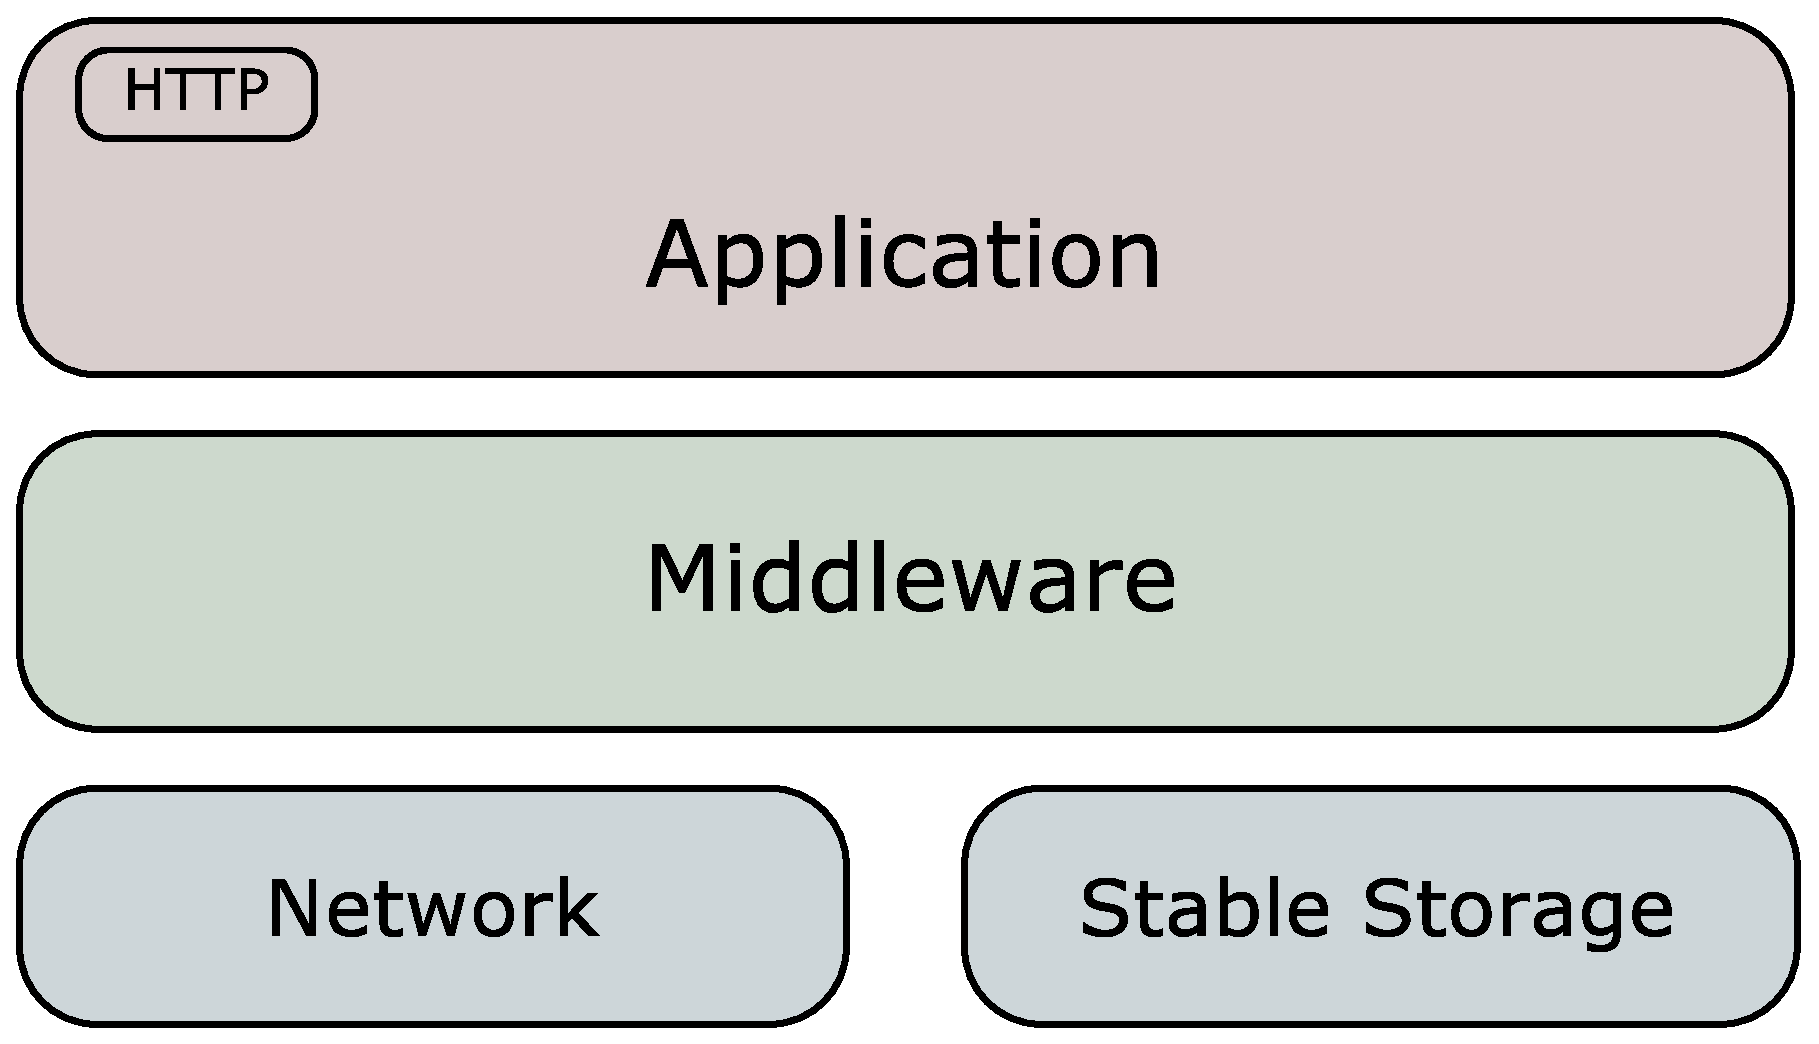
\includegraphics[width=12cm]{conteudo/capitulos/figuras/block-simple.eps}
  \caption{Separação em \emph{tiers}}
  \label{fig:tiers}
\end{figure}

Supomos que a uma aplicação que use replicação ativa o faz na forma de um servidor que
atende \emph{requisições} de \emph{clientes}. Esses clientes não têm conhecimento de como
as requisições são executadas. As réplicas recebem essa requisições e as processam de forma
a manter a consistência do estado replicado (compartilhado). Cada uma dessas requisições
executa o equivalente a uma chamada de função no contexto do estado da aplicação. Se a
função subjacente altera o estado, esta é uma \emph{requisição de escrita} e deve ser
difundida e ordenada entre todas as réplicas antes de ser executada. Caso a função
subjacente não altere estado, esta é uma \emph{requisição de leitura} e pode ser executada
localmente sem coordenação entre as réplicas.

\subsubsection{Layers}

Do ponto de vista da estruturação física para suportar a aplicação, supomos um conjunto de
réplicas que é gerenciada por um servidor balanceador de carga, usado para melhorar o
desempenho de serviços Web distribuindo requisições entre vários servidores. Todas as
requisições dos clientes passam pelo balanceador de carga, configurado para receber e
rotear as requisições para as réplicas ativas, usando um algoritmo de revezamento circular
(\emph{round-robin}), como ilustrado na \autoref{fig:layers}.

\begin{figure}[ht]
  \centering
  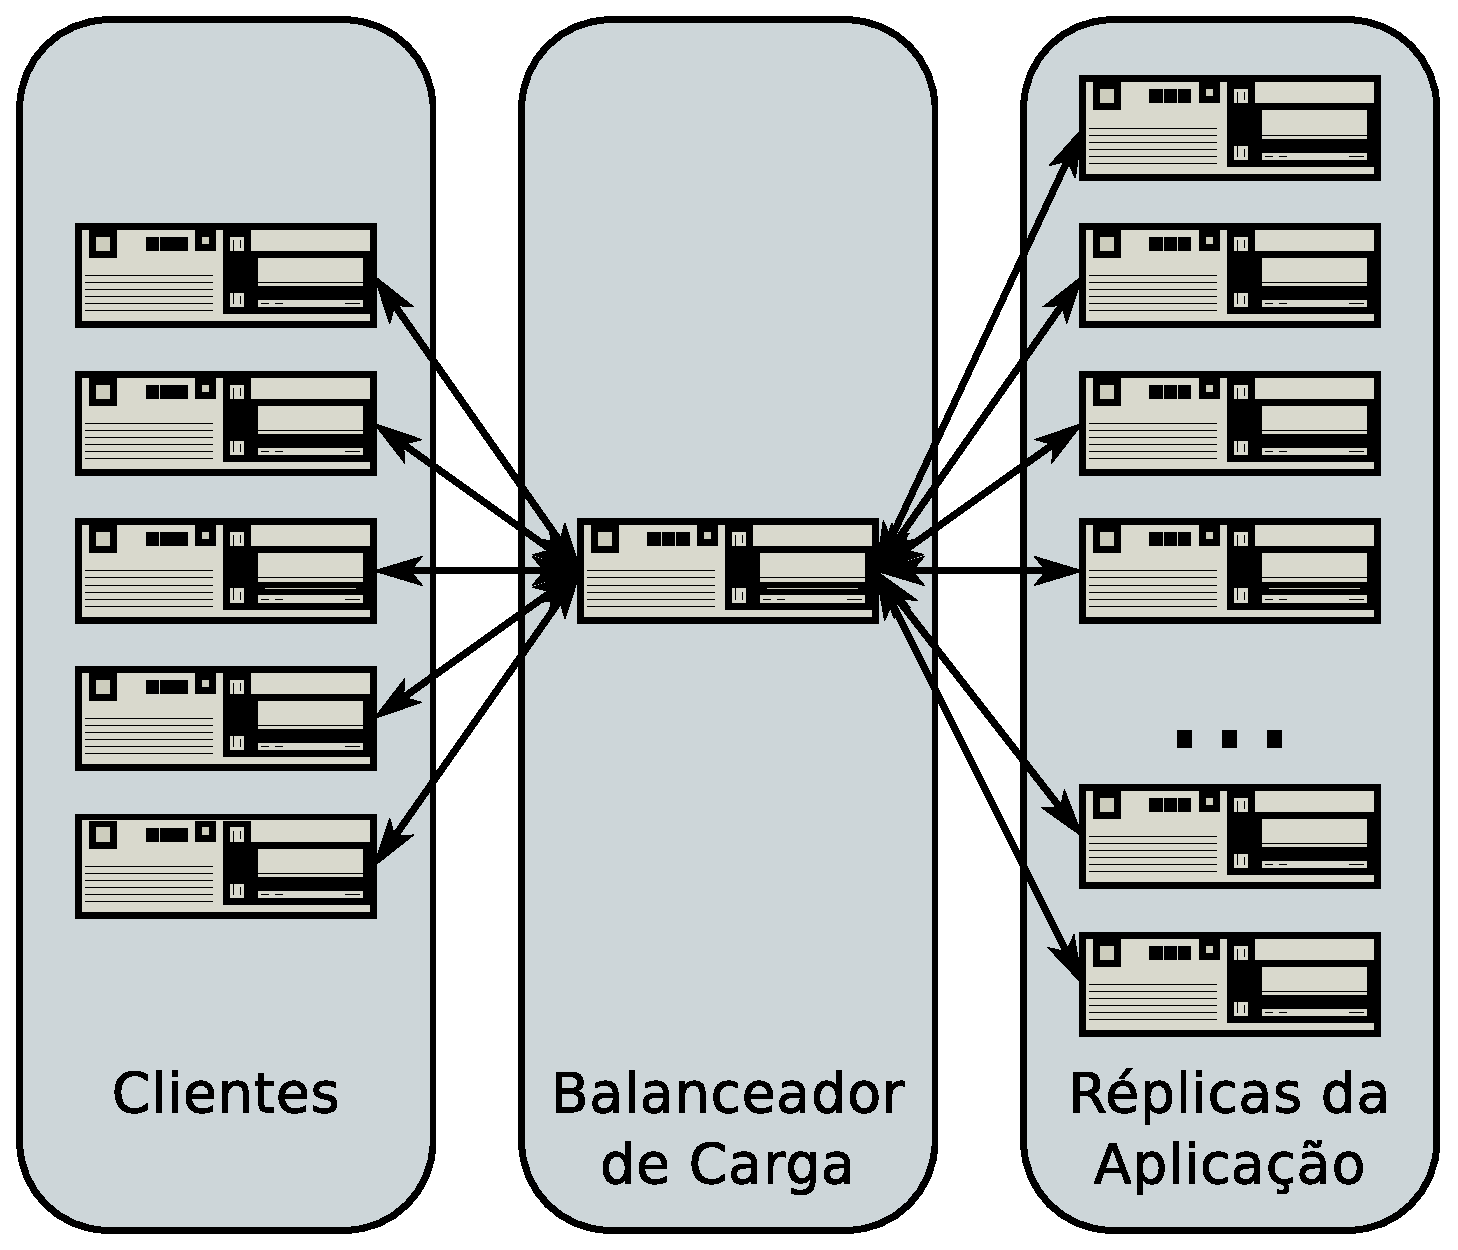
\includegraphics[width=10cm]{conteudo/capitulos/figuras/layers.eps}
  \caption{Separação em \emph{layers}}
  \label{fig:layers}
\end{figure}

O balanceador de carga monitora as réplicas para tentar detectar quando a aplicação está
disponível. Assim que uma réplica está disponível ela passa a receber requisições roteadas
pelo balanceador de carga. O monitoramento é realizado através de pequenos pacotes
\emph{keepalive} que são enviados para cada réplica do aglomerado. Todos os componentes
estão conectados através de um \emph{switch} que se comporta como uma canal de perda-justa.


\section{Replicação Ativa}\label{sec:replicacao-ativa}

Em geral, é uma boa ideia replicar serviços ou dados (estado) de uma aplicação. A
replicação é um mecanismo fundamental em sistemas distribuídos, proporciona maior
disponibilidade e ajuda a equilibrar a carga entre componentes, o que potencialmente
resulta em melhor desempenho \cite{tanenbaum07}. O acesso a serviços ou dados replicados
deve ser transparente para o usuário, ele deve ser realizado da mesma forma que o faria
como se não houvesse replicação. A consistência dos dados replicados deve ser garantido
automaticamente pelas réplicas e mesmo que mais de uma réplica responda a uma requisição,
apenas uma resposta deve ser entregue ao usuário final.

A criação de um grupo de réplicas minimiza a percepção de falhas de um cliente que acessa
um estado compartilhado. Entretanto, para que o grupo de réplicas seja transparente para
aplicação cliente, é preciso adotar uma estratégia de replicação a fim de coordenar as
réplicas preparando-as para que, no momento que ocorrer uma falha, uma réplica possa dar
continuidade ao processamento do sistema~\cite{jalote94}. Existem duas técnicas seminais
de replicação de processos: a \emph{replicação ativa} e a \emph{replicação passiva}
\cite{jalote94}. Esses modelos de replicação são capazes de tolerar falhas de maneira
transparente para o cliente, na ativa a escrita é garantida nas réplicas e na passiva a
escrita ocorrerá mais cedo ou mais tarde (futura).

Na replicação ativa \cite{coulouris11, guerraoui97} ou replicação por máquina de estados
\cite{schneider90}, os processos replicados funcionam como máquinas de estado
deterministas, ou seja, o estado atual é determinado única e exclusivamente por um estado
inicial e uma sequência de transições. Desta forma, se os processos replicados recebem a
mesma sequência de transições eles atingirão estados idênticos.

Cada operação que altera o estado de uma réplica (requisição de escrita) é executada de
maneira determinista no conjunto de réplicas, ou seja, todas as réplicas recebem e
processam a mesma sequência de requisições, conforme ilustrado na
\autoref{fig:write-replication}.

\begin{figure}[htbp]
  \centering
  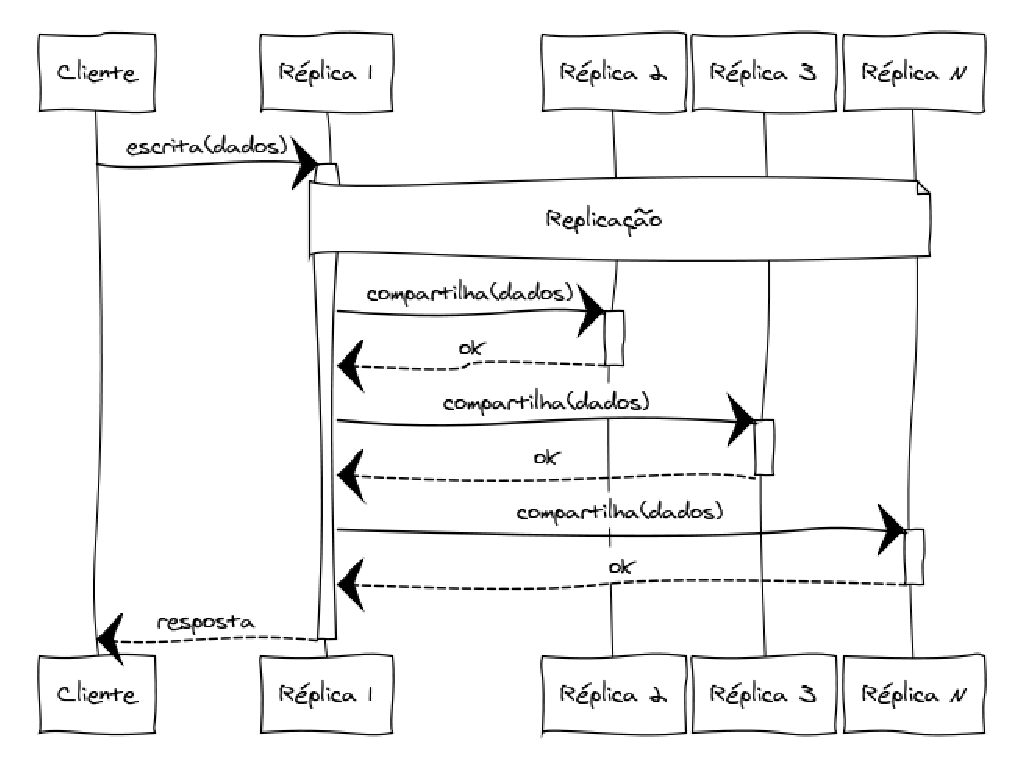
\includegraphics[width=14.5cm]{conteudo/capitulos/figuras/escrita_replicacao.eps}
  \caption{Requisição de escrita}
  \label{fig:write-replication}
\end{figure}

A propagação das requisições de mudança no conjunto de réplicas garante a sincronização
consistente global do estado, pois é replicando a atualização de estado sofrida por uma
réplica em todas as outras réplicas que uma requisição de leitura pode ser executada
localmente em qualquer réplica com a certeza do mesmo resultado. A
\autoref{fig:read-replication} ilustra esse cenário, repare que não existe propagação da
requisição para outras réplicas, a requisição e processada localmente.

\begin{figure}[htbp]
  \centering
  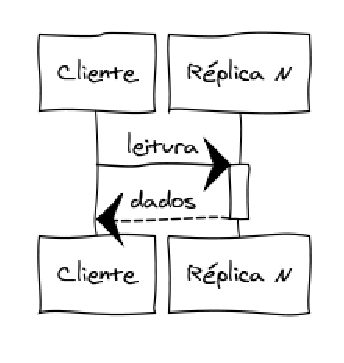
\includegraphics[width=6.5cm]{conteudo/capitulos/figuras/leitura_replicacao.eps}
  \caption{Requisição de leitura}
  \label{fig:read-replication}
\end{figure}

Não é necessário modelar o funcionamento de uma aplicação que use replicação ativa como
uma máquina de estados explícita, basta considerar as funções da aplicação que mudam o
estado como transições. As funções que não mudam o estado não têm correspondência na
abstração de máquina de estados, sendo simples consultas ao estado armazenado e não exigem
ordenação.

Uma desvantagem da replicação ativa é que por requerer réplicas deterministas ela
restringe o uso de múltiplos fluxos de execução (\emph{multithreading}) e outros
mecanismos que podem causar indeterminismos, mas que podem melhorar o desempenho. O
requisito de ordem total pode ser relaxado se as requisições dos clientes forem
comutativas ou idempotentes. Para um sistema $f-$tolerante a falhas, são necessários $f +
1$ réplicas ativas para garantir progresso da aplicação \cite{jalote94, lamport10}.
Requisições de escrita encarecem a aplicabilidade desse modelo, pois precisamos escrever
em um número grande o suficiente de réplicas de tal forma que a escrita não seja
esquecida.

Replicação ativa consistente é uma tarefa complicada e cara porque no modelo computacional
adotado não há uma ideia de relógio global compartilhado. Ou seja, processos em máquinas
diferentes têm sua própria ideia do que é o tempo e como ele passa, logo não podem
determinar com certeza se alguma das outras réplicas estão defeituosas. Para garantir a
consistência, as réplicas devem executar a mesma sequência de eventos, dessa forma é
possível manter o estado análogo em qualquer réplica, mesmo que o mesmo evento em máquinas
diferentes seja processado em momentos distintos \cite{tanenbaum07}. Ordenar as
requisições de forma única, na presença de falhas, é equivalente a resolver o problema de
consenso \cite{chandra96}.


\section{Paxos}\label{sec:paxos}

O algoritmo Paxos \cite{lamport98} é uma solução completa para replicação ativa usando
consenso. Paxos é destinado ao modelo assíncrono de computação com falha-e-recuperação que
utiliza detectores de falha imperfeitos. Em particular, ele garante que o estado de
nenhuma réplica irá divergir do das demais, mesmo na presença de falhas e de comportamento
assíncrono de processamento e canais de comunicação.

Paxos emprega um conjunto de protocolos baseados em quórum para atualizar os dados
replicados em um grupo. O objetivo do algoritmo é coordenar as réplicas para que todas
tenham o mesmo estado \cite{cachin11}. Para garantir o progresso e correção do algorítimo,
as seguintes propriedades são destacadas:

\begin{itemize}
  \item Validade Uniforme: se um processo decide $v$ então algum processo anteriormente
    propôs $v$.
  \item Acordo: não existem dois processos corretos que decidem valores diferentes.
  \item Encerramento: Se todos os processos corretos propõem um valor, então mais cedo ou
    mais tarde, eles serão decididos.
\end{itemize}

Por utilizar um mecanismo baseado em quórum, o algoritmo não depende de que todas as
réplicas estejam ativas para garantir que a escrita seja durável. Entenda por durabilidade
\footnote{Semelhante a propriedade ACID definida em transações de banco de dados
\cite{haerder83}} que uma vez que a transação foi confirmada, ela permanecerá assim, mesmo
em caso de falhas ou erros. Ou seja, os dados foram gravados em memória não-volátil.

\subsection{Algoritmo Básico}

Em Paxos os processos no sistema são agentes reativos que podem assumir vários
papéis: \emph{proponente} (\emph{proposer}) que pode propor valores, \emph{receptor}
(\emph{acceptor}) que escolhe um único valor ou \emph{aprendiz} (\emph{learner}) que
aprende o valor escolhido. Para resolver o consenso, agentes do Paxos executam várias
\emph{rodadas} (\emph{rounds}), onde cada rodada possui um \emph{coordenador}
(\emph{coordinator}) e é unicamente identificado por um inteiro positivo, o \emph{número
de rodada}. Proponentes enviam a sua \emph{proposta} para o coordenador que tenta alcançar
consenso sobre a proposta em uma rodada, sendo que cada proposta corresponde a uma ou mais
requisições de escrita da aplicação sendo replicada.

O coordenador é responsável por essa rodada e executa um número definido de passos de
comunicação para garantir que a decisão tomada nessa rodada seja aceita pelos demais
processos, ou seja, um consenso. Este agente de Paxos é capaz e decidir, após aplicar uma
regra local, se outras rodadas tiverem sucesso ou não. A regra local do coordenador é
baseada em quóruns de receptores e exige que pelo menos $\lfloor n/2 \rfloor + 1$
receptores façam parte de uma rodada, onde $n$ é o número total de receptores na
aplicação \cite{lamport98}.

Cada rodada acontece em duas fases, com dois passos cada, como ilustrado na
\autoref{fig:fases-paxos}:

\begin{itemize}
  \item Na Fase 1a o coordenador envia uma mensagem convidando todos os receptores a
    participar de uma rodada $r$. Um receptor aceita o convite apenas se ele não aceitou
    participar de uma rodada $s \geq r$. Caso contrário, ele ignora o convite.
  \item Na Fase 1b todo receptor que aceitou o convite responde ao coordenador informando
    a última proposta votada por esse receptor e a rodada em que esse voto ocorreu, ou
    \textsl{null} se ele nunca votou.
  \item Na Fase 2a, se o coordenador da rodada $r$ recebeu respostas de um quórum de
    receptores, ele analisa o conjunto de respostas recebidas e escolhe uma proposta $p$
    que foi ou que poderia ter sido decidida em rodadas com número menor que $r$. Ele
    então pede a esses receptores para votar nessa proposta, ou caso ela seja
    \textsl{null}, para votar em uma das propostas feitas pelos proponentes.
  \item Na Fase 2b, após receber um pedido para votar do coordenador, receptores votam na
    proposta sugerida se eles não votaram em nenhuma rodada $s \geq r$. Os receptores
    votam enviando o número de rodada e a proposta aos aprendizes.
  \item Finalmente, um aprendiz descobre que uma proposta $p$ foi escolhida se ele receber
    mensagens da Fase 2b de um quórum de receptores, todos votado em $p$ na mesma rodada
    $r$.
\end{itemize}

\begin{figure}[htbp]
  \centering
  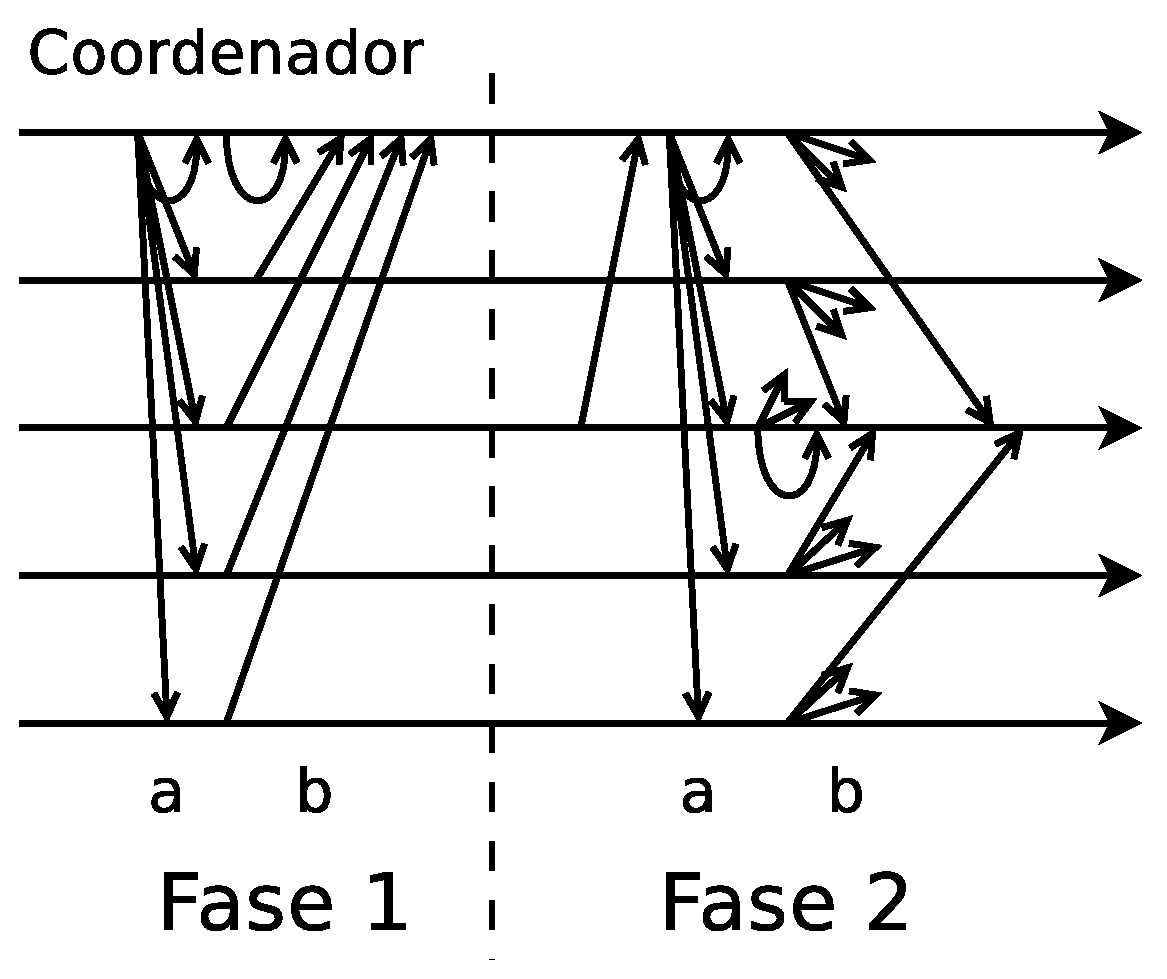
\includegraphics[width=9cm]{conteudo/capitulos/figuras/paxos.dia.eps}
  \caption{Paxos}
  \label{fig:fases-paxos}
\end{figure}

Cada rodada corresponde à decisão de uma proposta apenas. Porém Paxos define também uma
forma de entregar um conjunto de requisições de escrita totalmente ordenadas. A ordem de
entrega dessas requisições é determinada pela sequência dos inteiros positivos, tal que
cada inteiro corresponde uma \emph{instância} de consenso. Cada instância $i$ terá um
valor decidido, que corresponde a $i$-ésima requisição (ou conjunto ordenado de
requisições) a ser executada na sequência de requisições. Cada instância de consenso é
independente das demais e várias instâncias podem estar em curso ao mesmo tempo.

Como Paxos é definido no modelo falha-e-recuperação assíncrono, esse algoritmo exige que
os agentes armazenem estado em memória não volátil \cite{lamport06a}. Esse estado é
composto por um registro das instâncias iniciadas, os números de rodadas usados e as
propostas feitas e votadas, entre outros dados. De forma resumida, o coordenador escreve
na memória persistente na Fase 1a e os receptores o fazem nas Fases 1b e 2a. Não há a
necessidade de que a proposta decidida seja registrada para garantir a correção do
algoritmo, mas isto é normalmente feito para acelerar a recuperação. A escrita de dados em
memória persistente faz parde do caminho crítico de desempenho da execução das duas fases
do algoritmo Paxos. Logo, dependendo do custo de comunicação de rede, esse é o principal
gargalo de desempenho para a execução de Paxos.

Em Paxos, qualquer processo pode agir como o coordenador de uma rodada enquanto ele seguir
a regra para escolher uma proposta coerente como o resultado das rodadas anteriores na
Fase 2a. A escolha do coordenador e a decisão de iniciar uma nova rodada de consenso são
feitas com base em algum mecanismo de temporização, uma vez que Paxos supõe um modelo
computacional parcialmente síncrono para garantir progresso (\emph{liveness}).
Especialmente, a todo momento deve existir apenas um coordenador ativo para garantir que o
algoritmo progrida. Se dois ou mais processos iniciam agentes coordenadores, o algoritmo
pode travar enquanto estes múltiplos coordenadores competem pela atenção dos receptores
com números de rodada que crescem rapidamente. Por esta razão, o progresso do algoritmo
depende de um procedimento de seleção de coordenador. Este procedimento não precisa ser
perfeito. A correção do algoritmo nunca é comprometida se zero ou mais coordenadores
estiverem ativos ao mesmo tempo. Porém, o procedimento de seleção de coordenador deve ser
robusto o suficiente para garantir que apenas um único coordenador esteja ativo a maior
parte do tempo.

\subsection{Recuperação}

Uma consideração em relação ao funcionamento típico de Paxos é o que acontece
quando uma réplica inicia depois que o sistema já está operando ou quando reinicia após
uma falha prolongada. Esse caso não é explicitamente definido na descrição clássica de
Paxos, porém o algoritmo permite que um número arbitrário de rodadas aconteçam
\emph{antes} ou \emph{depois} que o consenso seja alcançado \cite{lamport98}. Dessa forma,
podemos supor um mecanismo de recuperação simples onde uma réplica que ficou fora de
operação por algum tempo atualiza o seu estado pela decisão sucessiva das instâncias de
consenso que ela não tem conhecimento. Esse mecanismo é apropriado para pequenas
interrupções, como a perda de algumas mensagens ou uma falha transiente. Porém, caso uma
réplica tenha um grande estado para atualizar esse procedimento pode ter impacto adverso
no desempenho do sistema.

Para exemplificar o possível impacto cenário de recuperação, vamos supor as seguintes
propriedades relacionadas a atualização de uma réplica desatualizada:

\begin{itemize}
  \item Consistência: Uma réplica desatualizada $r$ volta a computação após $n$ rodadas de
    consenso, onde $n$ é um número arbitrariamente grande. Se $r$ aplicar as $n$ decisões
    de consenso sucessivamente atingirá o mesmo estado das demais réplicas.
  \item Volatilidade do estado: Se o número de rodadas de consenso $n$ muda em uma
    velocidade maior que a réplica desatualizada $r$ consegue atualizar seu estado, $r$
    estará sempre desatualizada \cite{vilaca09}.
\end{itemize}

Baseado nessas propriedades de consistência e volatilidade não podemos afirmar nada com
relação ao tempo de recuperação de estado de uma réplica. O mecanismo de recuperação por
aplicação de decisões de consenso é ineficiente quando uma réplica possui um estado muito
antigo. Para atendermos eficientemente este cenário, precisamos de uma nova política de
recuperação. Uma alternativa é transferir para a réplica desatualizada o estado de uma
réplica atualizada, dessa forma supriremos a lacuna de desatualização substituindo por
completo o estado desatualizado por um atualizado, semelhante a ideia de um transplante.

\subsection{Estado persistente}

Para satisfazer as propriedades de consenso no modelo falha-e-recuperação assíncrono é
preciso utilizar um mecanismo capaz de gravar dados de forma persistente (não-volátil).
Dessa forma, após um período de instabilidade uma réplica é capaz de recuperar suas
decisões de consenso tomadas anteriormente para continuar participando corretamente do
protocolo. A cada fase do algoritmo acontecem dois acessos a disco, conforme ilustrado na
\autoref{fig:fases-paxos-acesso-disco}

\begin{figure}[htbp]
  \centering
  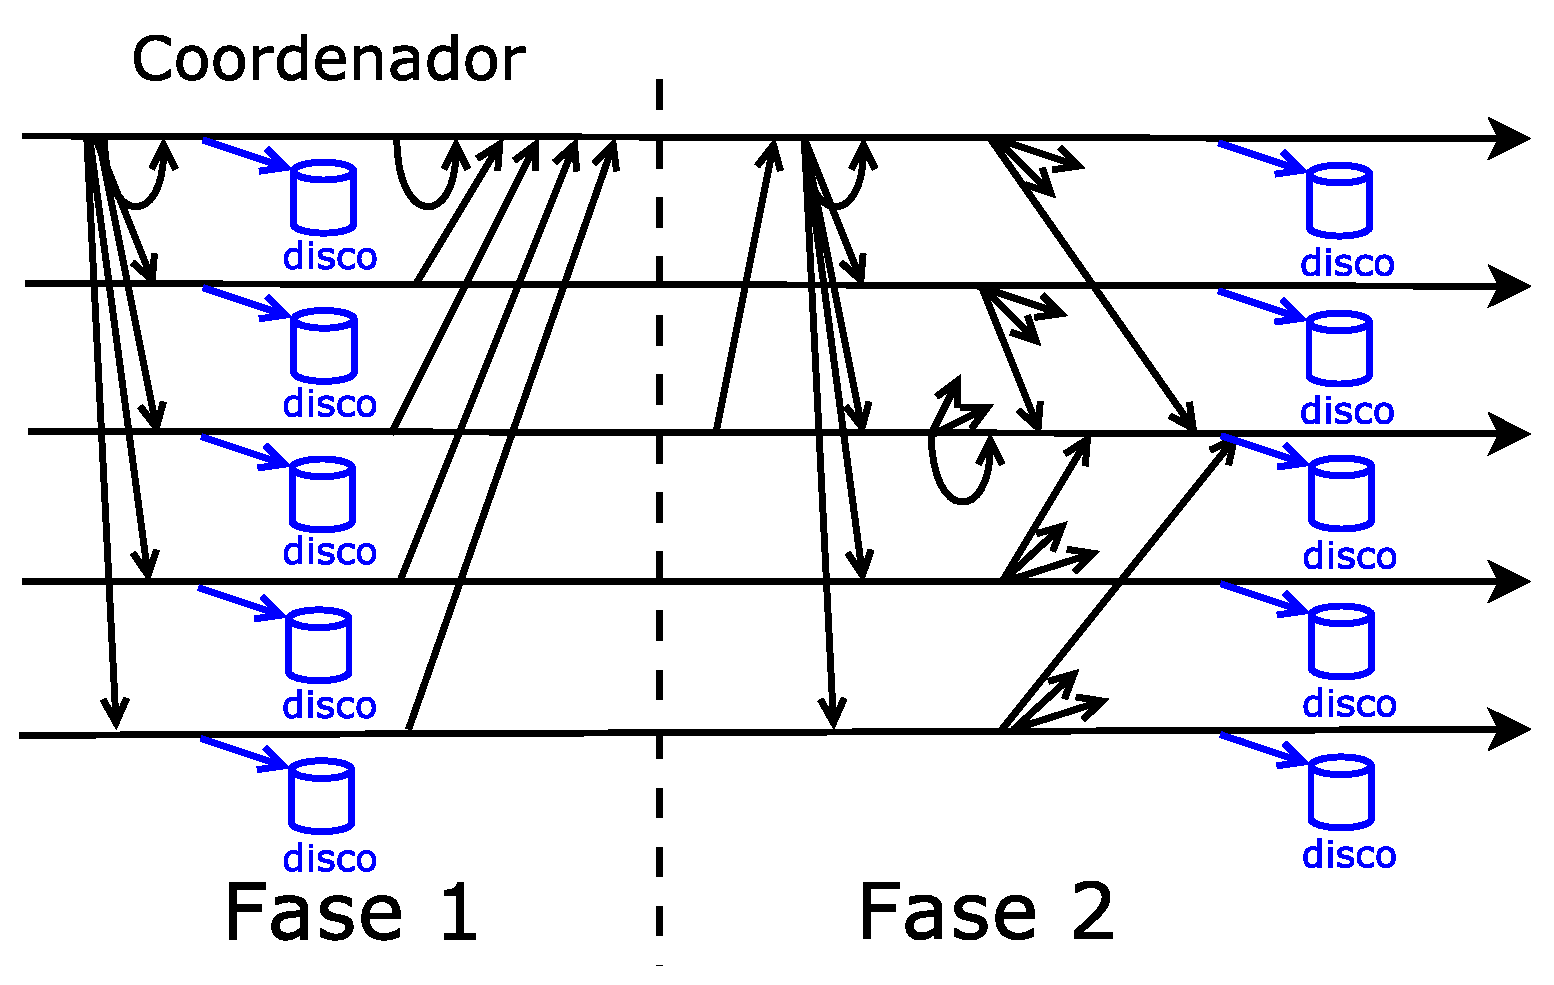
\includegraphics[width=9cm]{conteudo/capitulos/figuras/fases-paxos-acesso-disco.eps}
  \caption{Paxos}
  \label{fig:fases-paxos-acesso-disco}
\end{figure}

\begin{itemize}
  \item Na Fase 1, após receber um convite do coordenador para participar da rodada $r$,
    todo receptor que aceitou o convite, escreve $r$ em disco.
  \item Na Fase 2, toda a proposta $p$ que consegue estabelecer consenso em $r$ é
    escrita em disco. Ao final de cada rodada, foi persistido em disco o par (rodada,
    decisão).
\end{itemize}

Operações de persistência durável é custosa e tem grande potencial para reduzir o
desempenho do algoritmo. Por exemplo, considere que cada operação de escrita em disco leva
cerca de $1ms$ para ser concluída e que uma rodada de Paxos, pelo menos, requer duas
escritas em memória estável, acabamos de adicionar uma latência de $2ms$ em todas as
rodadas de consenso. \citeonline{aguilera00} propõem a combinação de réplicas com
diferentes graus de uso de memória persistente para diminuir o custo do armazenamento dos
dados. Essa proposta, através de vários teoremas, mostra que se o número de processos que
nunca falham é maior que o número de processos que eventualmente permanecem defeituosos ou
falham e se recuperam infinitamente, então o consenso pode ser resolvido sem armazenamento
persistente.

Esse trabalho apresenta a resolução de consenso nesse modelo com um número variável de
réplicas com memória persistente, desde que seja sempre possível entrar em contato com
uma réplica que use memória persistente ou com uma réplica sem memória persistente que
nunca falhe. Nossa proposta de replicação aplica-se para o algoritmo Paxos, determinando
que os quóruns responsáveis pelo consenso sejam sempre compostos por réplicas que usam
memória persistente.


\section{Treplica}\label{sec:treplica}

Treplica se situa a meio caminho entre flexibilidade de baixo nível de um sistema de
comunicação em grupo \cite{birman93} baseado em sincronia virtual \cite{friedman96,
birman05} e os vastos recursos de processamento de dados de um SGBD. A principal
característica de Treplica é a ideia de se apresentar ao programador como uma abstração de
programação unificada para replicação e persistência, propondo o uso de consenso
\cite{barborak93} como a fundação para a construção dessa ferramenta.

Treplica foi projetada para prover uma forma simples e orientada a objetos de se construir
aplicações altamente confiáveis. Essas aplicações podem se estender ao sistema inteiro ou
se restringir à subsistemas onde o desempenho, consistência e confiabilidade são cruciais.
Para alcançar esse objetivo, Treplica decompõe o problema de se implementar replicação em
componentes com interfaces simples e bem definidas.

Dessa forma, um desenvolvedor que deseje implementar uma aplicação distribuída não precisa
pensar em termos de processos, mensagens e falhas. Ao invés disso, ele pensa sobre a
execução das operações da aplicação, transições de uma máquina de estados replicada, que
são disparadas por eventos disponibilizados através de uma fila persistente assíncrona
\cite{vieira-tr10b}. A \autoref{fig:treplica} mostra a interface destes componentes e sua
relação com a aplicação e entre si.

\begin{figure}[ht]
  \begin{center}
    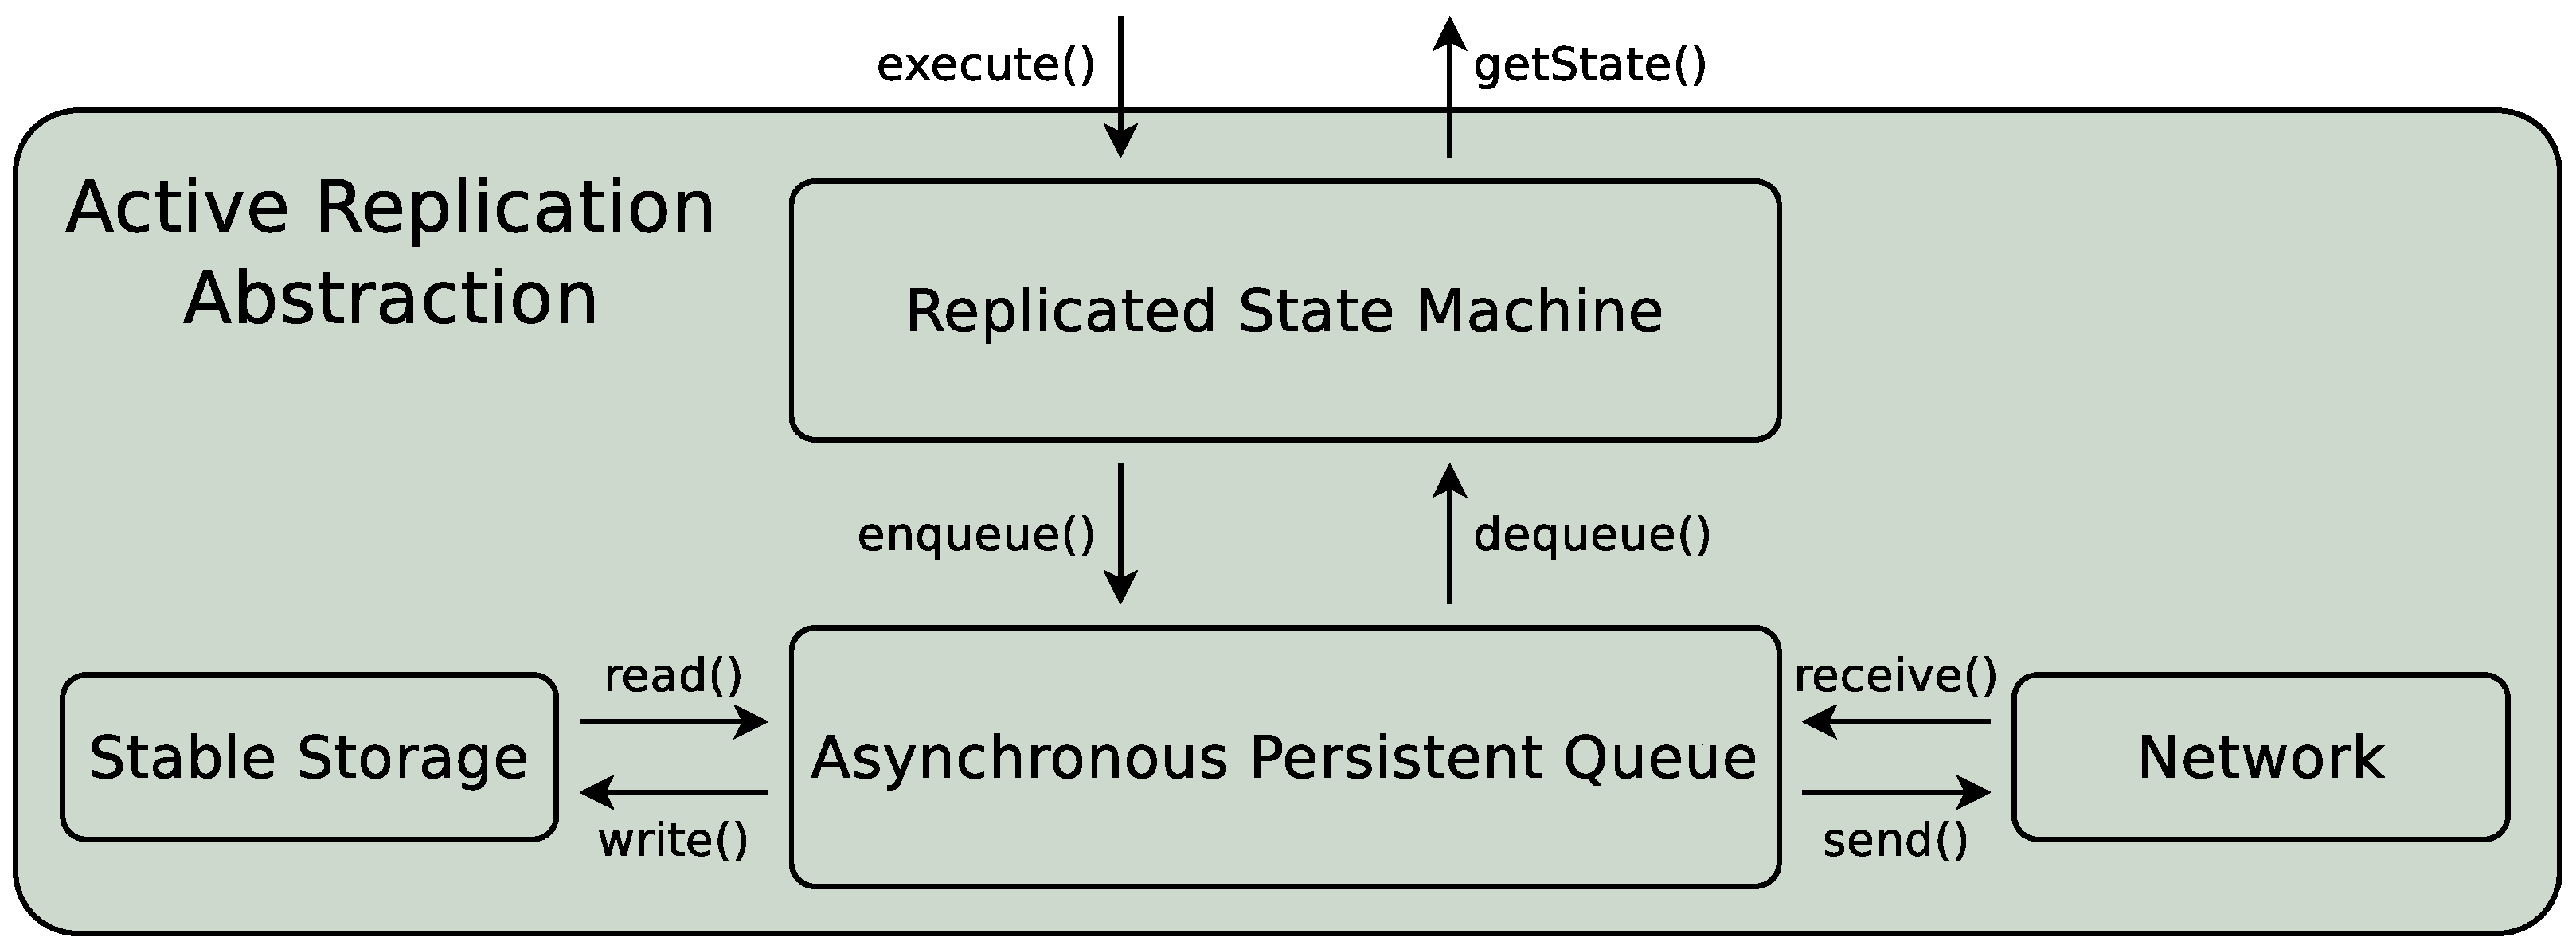
\includegraphics[width=14cm]{conteudo/capitulos/figuras/treplica.eps}
  \end{center}
  \caption{Componentes para replicação}
  \label{fig:treplica}
\end{figure}

A principal decisão de projeto por trás de Treplica é que o programador pode considerar a
sua aplicação como não tendo estado persistente, ficando a durabilidade da mesma garantida
pela biblioteca. Essa decisão é suportada pela observação que os mesmos requisitos de
replicação ativa podem ser usados para prover um mecanismo simples e poderoso de
persistência.

A replicação ativa exige que a aplicação execute ações que modificam o seu estado de forma
determinista. Essas ações são então propagadas, na mesma ordem, para todas as réplicas de
um serviço que as reexecutam localmente. Dentro dessa organização, as ações não são apenas
enviadas para as outras réplicas, mas arquivadas em memória estável \cite{birrel87}. Dessa
forma, é possível se recuperar de uma falha reexecutando o arquivo de ações. O
determinismo garante que após cada recuperação a aplicação reiniciará com o mesmo estado
que possuía antes da falha. Por razões de eficiência, a aplicação deve caber inteiramente
em memória principal, pois a biblioteca não armazena a aplicação em si, apenas mudanças de
estado.

A máquina de estados replicada provê uma abstração da operação de qualquer aplicação
determinista. Ela permite a manutenção do estado da aplicação estipulando uma interface
simples para consultar e modificar esse estado. Esse componente é acessado diretamente
pela aplicação que usa os seus serviços para armazenar, replicar e persistir o seu estado.
Todas essas operações são realizadas de forma transparente e não exigem intervenção por
parte do usuário desse componente.

A fila persistente assíncrona é uma abstração de uma fila de objetos persistentes e
tolerante a falhas. Ela representa um registro ordenado de objetos enviados a um grupo de
processos, que é garantidamente disponível mesmo se todos os processo deste grupo falhem.
Ela pode ser usada como um registro persistente dos eventos que disparam transições na
máquina de estados distribuída e é implementada usando algum mecanismo de difusão ordenada
de mensagens, como Paxos descrito na \autoref{sec:paxos}.


\section{Reconfiguração}\label{sec:reconfiguracao}

O processo de modificar o conjunto de réplicas que compõem o sistema chama-se
\emph{reconfiguração}. Alterar o número de réplicas participantes de uma aplicação que
utiliza o modelo de replicação ativa não é uma tarefa trivial pois a informação de
\emph{cardinalidade} do conjunto de réplicas é relevante para o mecanismo de replicação
gerenciar a consistência do estado compartilhado. Segundo \citeonline{lamport10}
reconfigurar é custoso, pois o algoritmo  Paxos trabalha com consenso e para que uma
rodada de consenso ocorra é preciso que o número de réplicas participantes seja claramente
definido. Isso obriga que cada expansão ou redução do grupo de réplicas seja precedido de
reconfiguração.

Paxos trabalha com protocolos baseados em quóruns, então a retirada de uma réplica da
computação sem a devida reconfiguração afeta diretamente o funcionamento correto do
algoritmo que foi projetado para trabalhar com um grupo estático de réplicas
\cite{chandra96, lamport98}, onde não é permitida a entrada e saída de servidores durante
a execução. Essa abordagem não é adequada para sistemas que permanecerão em execução por
um longo tempo, pois limitam a atuação de um administrador, que em tempo de execução, não
pode adicionar máquinas no sistema (para suportar um aumento na carga de processamento) ou
trocar máquinas antigas (para efetuar um reparo no hardware) \cite{alchieri14}. Oferecer
suporte a esses requisitos caracteriza, em sua forma mais simples, um comportamento
elástico que a aplicação deve suportar para refletir mudanças do ambiente operacional
durante o período de execução.

Para formar uma maioria que votou em uma mesma proposta é preciso que o mecanismo de
decisão de consenso conheça o número exato de réplicas em uma determinada rodada. Por
exemplo, caso existam apenas $\lfloor n/2 \rfloor + 1$ potenciais replicas e uma réplicas
$r$ for removido de forma ingênua, a formação legítima de quóruns não é mais possível.
Nesse caso, réplicas corretas serão levadas a 1) suspeitar indevidamente que $r$ falhou,
mas na realidade $r$ não pertence mais ao grupo de réplicas; 2) esperar indefinidamente
por uma resposta de $r$ para determinar a maioria. Essa espera indevida pode impedir a
progresso do algoritmo.

Por outro lado, uma aplicação configurada para executar com $n$ réplicas não pode
adicionar uma nova réplica de forma arbitrária sem ser precedida de reconfiguração. Caso
existam $n + 1$ réplicas ativas, a formação de um quórum que contenha todas as decisões de
consenso pode não ser mais verdade, pois não podemos mais garantir interseção de consenso
no conjunto de réplicas. Dessa forma afetamos diretamente a correção do algoritmo.

Para oferecer o dinamismo necessário na \emph{ampliação} e \emph{redução} de grupos
de réplicas em sistemas distribuídos modernos, \citeonline{lamport10} propõem a criação de
um mecanismo de visões. Nessa proposta uma nova visão $v$ do sistema é criada sempre que uma
réplica $r$ for adicionada ou retirada da computação. Nessa visão $v$, $r$ pode fazer
parte ou não do processamento computacional, dependendo da operação executada. Durante a
execução de uma aplicação, ela pode passar por diferentes visões (configurações) sem
afetar seu progresso e correção, mas sistemas práticos tendem a evitar essa questão de
forma a simplificar a construção de aplicações \cite{chandra07}.

Projetar mecanismos autônomos capazes de realizar reconfiguração, sintonizados para reagir
rapidamente às mudanças do sistema e gerar novas réplicas com base no uso de recursos e
medidas de desempenho, é um assunto atual e relevante para pesquisa. Por outro lado,
estamos preocupados com o impacto inerente de implantar uma nova réplica em um aglomerado
em tempo de execução. Se perceptível tal impacto dificulta a viabilidade das técnicas de
autogestão, porque dependendo do cenário adicionar uma nova réplica pode comprometer o
desempenho de um sistema sobrecarregado \cite{vilaca09}.

Segundo o estudo de \citeonline{vilaca09}, a política de reconfiguração deve levar em
consideração a velocidade das mudanças de estado da aplicação no momento que deseja
reconfigurá-la. Isso  ocorre  pois quando a eficiência da transferência é menor que a
velocidade de mudanças no estado, a nova réplica  nunca receberá o estado mais atual da
aplicação podendo não participar das rodadas atuais de consenso.

Então temos dois problemas em mãos: (1) alterar o numero de réplicas sem violar o
progresso do algoritmo quando remover réplicas e a correção do algoritmo quando adicionar
réplicas. Dessa forma prover uma capacidade elástica preservando a consistência de Paxos;
(2) provisionar réplicas de forma que não comprometa o desempenho, aumentando o suporte
aos picos de acesso, denominados \emph{flash crowds}, existentes na Internet
\cite{tanenbaum07}.


\section{Trabalhos Relacionados}\label{sec:trabalhos-relacionados}

A ideia de se combinar réplicas com diferentes graus de uso de memória persistente no
modelo falha-e-recuperação assíncrono foi formalizada por \citeonline{aguilera00}. Para
esse trabalho supomos a resolução de consenso nesse modelo, utilizando o algotimo Paxos
com um número variável de réplicas que possuem memória persistente. Estabelecemos a forte
premissa que os quóruns responsáveis pelo consenso sejam sempre compostos por réplicas que
usam memória persistente.

Do ponto de vista de engenharia de sistemas, a nossa proposta se assemelha às arquiteturas
de cache distribuídas. Um exemplo notável é o Mencached
\footnote{\url{http://memcached.org/}} que é um repositório de chave/valor. Esse sistema é
usado para armazenar, de forma distribuída pelo aglomerado, dados que podem que a
aplicação faça consultas custosas a um banco de dados centralizado. Usando Mencached o
projetista de aplicação deve modificar o seu programa para registrar as informações úteis
para atender requisições de leitura no cache distribuído. De forma similar, a nossa
proposta procura evitar que seja feito acesso a um recurso nobre, nesse caso as réplicas
votantes. Porém, o uso de réplicas leitoras é transparente ao programador de aplicação que
não precisa se preocupar em particionar os seus dados entre aqueles que são armazenáveis
no cache e aqueles que não são.

Um outro sistema que faz uso extensivo de cache é o gerenciador de bloqueios distribuídos
Chubby \cite{burrows06} usado no Google. Nesse sistema o número de réplicas que fornecem o
serviço é fixo e relativamente pequeno (5 réplicas), e os clientes acessam o serviço
apenas através de uma réplica mestre. A chave para o desempenho desse sistema é o fato de
que os clientes acessam o serviço usando uma biblioteca especial que constrói um cache
local, usando \emph{leases} regidos por tempo \cite{lampson96} para garantir a
consistência dos mesmos. Em comparação, a nossa proposta não exige um cliente especial, o
que a torna mais indicada para aplicações em geral, especialmente no ambiente Web. Dessa
forma, temos uma implementação de cache que também é transparente ao cliente que acessa a
aplicação.

